\documentclass{ctexart}
\usepackage[left=1.5cm,right=1.5cm,top=1.5cm,bottom=1.5cm]{geometry}
\usepackage{listings}
\usepackage[dvipsnames]{xcolor}
\usepackage{cite}
\usepackage{diagbox}
\usepackage{fancyhdr} % 加载fancyhdr宏包,用于设置页眉和页脚
\pagestyle{fancy} % 设置页面样式
\fancyhf{} % 清除默认的页眉和页脚的内容
\fancyfoot[C]{\thepage} 
\renewcommand{\headrulewidth}{0pt} % 将页眉的横线宽度设置为0pt

\usepackage{graphicx}
\usepackage{longtable}
\usepackage{tabularx}
\usepackage{float}
\usepackage{amsmath}%引用宏包要放在documentclass后面,否则报错
\usepackage{hyperref}
\usepackage{bm}
\usepackage{amssymb}
\usepackage{esint}
\usepackage{booktabs}
%\usepackage{subfiles}%用于分章节管理引用,使各章节引用来源于各自的文件,编号相互独立
\usepackage{amsthm}
\title{数字电路实验\quad 实验报告8}
\author{Leo}
\date{\today}
\begin{document}
\maketitle
\section{实验内容}
\noindent 使用LED设计一种彩灯花灯:\\
1.选取并熟悉相关芯片\\
2.列出状态转移真值表和转换图 \\
3.给出电路实现方案\\
4.调试电路,实现控制8路LED以2种速度(0.5秒和1秒)连续显示3种显示式样。两种速度交替进行,彩灯花型为:\\
a.	依次点亮,反序熄灭;\\
b.	两边到中间依次点亮,反序熄灭;\\
c.	两个灯亮右移\\
\section{实验器材}
Pocketlab、电脑、导线若干、镊子、限流电阻1个、黄色LED灯4个、绿色LED灯4个、7400*2、7404*2、7420*3、74138*3、74194*2、74191*1、7474*1。芯片的引脚图如下所示
\begin{figure}[H]
    \centering
    \begin{minipage}{0.45\textwidth}
    \centering
           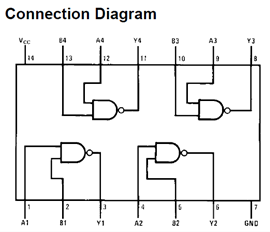
\includegraphics[width=0.6\textwidth]{7400.png}
           \caption{7400}
    \label{}
    \end{minipage}
    \hspace{0.05\textwidth}
    \begin{minipage}{0.45\textwidth}
    \centering
           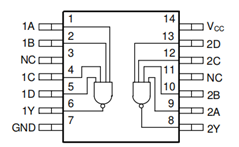
\includegraphics[width=0.6\textwidth]{7420.png}
           \caption{7420}
    \label{7474}
    \end{minipage}
\end{figure}
\begin{figure}[H]
    \centering
    \begin{minipage}{0.5\textwidth}
    \centering
           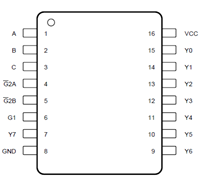
\includegraphics[width=0.5\textwidth]{74138.png}
           \caption{74138}
    \label{}
    \end{minipage}
    \hspace{0.05\textwidth}
    \begin{minipage}{0.4\textwidth}
    \centering
           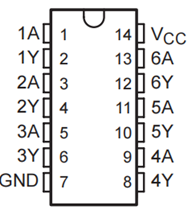
\includegraphics[width=0.5\textwidth]{7404.png}
           \caption{7404}
    \label{7474}
    \end{minipage}
\end{figure}
\begin{figure}[H]
    \centering
    \begin{minipage}{0.45\textwidth}
    \centering
           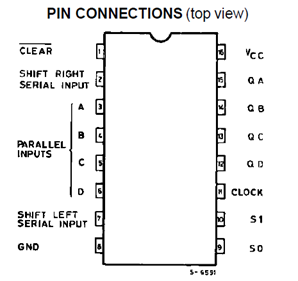
\includegraphics[width=0.6\textwidth]{74194.png}
           \caption{74194}
    \label{}
    \end{minipage}
    \hspace{0.05\textwidth}
    \begin{minipage}{0.45\textwidth}
    \centering
           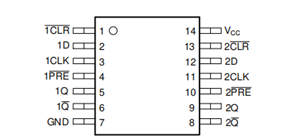
\includegraphics[width=0.9\textwidth]{7474.png}
           \caption{7474}
    \label{7474}
    \end{minipage}
\end{figure}
\begin{figure}[H]
    \centering
    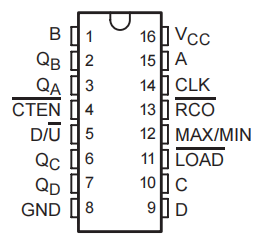
\includegraphics[width=0.25\textwidth]{74191.png}
    \caption{74191}
\end{figure}
\section{实验原理}
题目中的三种花型与移位寄存器的工作状态比较相似,所以考虑用移位寄存器的输出端作为灯的输入。针对三种花型,可以将其描述为16种状态。其中,前八种状态可以表述为
\begin{enumerate}
    \item 右移“1”,持续8个时钟周期
    \item 左移“0”,持续8个时钟周期
    \item 低位的移位寄存器右移“1”,高位左移“1”,持续4个时钟周期
    \item 低位的移位寄存器左移“0”,高位右移“0”,持续4个时钟周期
    \item 低位送数到$Q_A Q_B$,持续1个时钟周期
    \item 低位送数到$Q_C Q_D$,持续1个时钟周期
    \item 高位送数到$Q_A Q_B$,持续1个时钟周期
    \item 高位送数到$Q_C Q_D$,持续1个时钟周期
\end{enumerate}
其中,第一二种状态对应花型a,第三四种状态对应花型b,后四种状态对应花型c。每一个时钟周期为0.5s。没有列出的后八种状态类似,只是每一个时钟周期为1s。所以,电路一共有16种状态。现在对状态进行编码。如图所示
\begin{figure}[H]
    \centering
    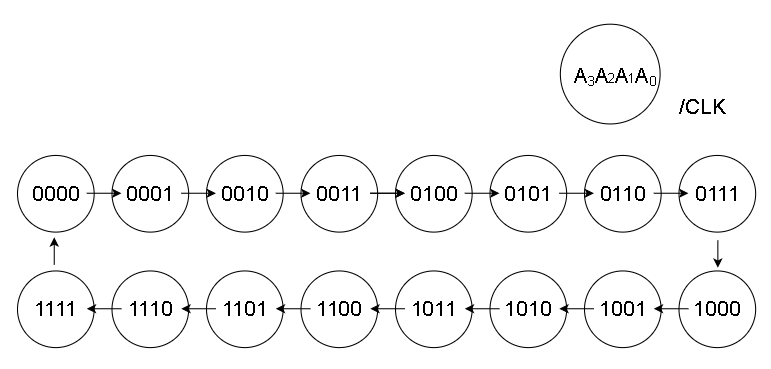
\includegraphics[width=0.6\textwidth]{状态转换图.png}
    \caption{状态转换图}
\end{figure}
可以发现,这种编码方式适合由二进制计数器来实现,故选择74191作为状态转移模块,且一共有16种状态,对于4位的74191来说,没有偏离状态,可以自启动。进一步观察发现,16种状态中,最高位$A_3$负责选择速度,后三位$A_2 A_1 A_0$负责选择花型。这样就实现了选速与选花功能的分离,即选花与$A_3$不直接相关,选速与$A_2 A_1 A_0$不直接相关。下面先来实现选择花型的功能。

花型的选择,实际上是移位寄存器置数方式和移位方式的选择,即:左移、右移和直接置数的选择。这由74194的$S_1 S_0$和$S_L S_R$来控制。由于选花只与$A_2 A_1 A_0$直接相关,所以只列出$S_1 S_0$和$S_L S_R$与$A_2 A_1 A_0$的关系。记低位移位寄存器的移位控制端为$S_{11},S_{10},S_{R1},S_{L1}$,高位移位寄存器的移位控制端为$S_{21},S_{20},S_{R2},S_{L2}$.列出真值表
\begin{table}[H]
    \centering
    \caption{移位控制端的真值表}
    \begin{tabular}{ccc|cccc|cccc}
    \hline 
        $A_2$ & $A_1$ & $A_0$ & $S_{11}$ & $S_{10}$ & $S_{21}$ & $S_{20}$ & $S_{R1}$ & $S_{L1}$ & $S_{R2}$ & $S_{L2}$\\ \hline 
        0 & 0 & 0 & 0 & 1 & 0 & 1 & 1 & x & $Q_{1 D}$ & x \\ \hline
        0 & 0 & 1 & 1 & 0 & 1 & 0 & x & $Q_{2 A}$ & x & 0 \\ \hline
        0 & 1 & 0 & 0 & 1 & 1 & 0 & 1 & x & x & 1 \\ \hline
        0 & 1 & 1 & 1 & 0 & 0 & 1 & x & 0 & 0 & x \\ \hline
        1 & 0 & 0 & 1 & 1 & 1 & 1 & x & x & x & x \\ \hline
        1 & 0 & 1 & 1 & 1 & 1 & 1 & x & x & x & x \\ \hline
        1 & 1 & 0 & 1 & 1 & 1 & 1 & x & x & x & x \\ \hline
        1 & 1 & 1 & 1 & 1 & 1 & 1 & x & x & x & x \\ \hline
    \end{tabular}
    \label{移位控制端的真值表}
\end{table}
根据真值表可以画出卡诺图
\begin{figure}[H]
    \centering
    \begin{minipage}{0.5\textwidth}
    \centering
    \begin{table}[H]
        \centering
        \caption{$S_{11}$的卡诺图}
        \begin{tabular}{|c|c|c|c|c|}
    \hline
    \diagbox{$A_2$}{$A_1 A_0$} & 00 & 01 & 11 & 10 \\
    \hline
    0 & 0 & 1 & 1 & 0 \\
    \hline
    1 & 0 & 0 & 0 & 0  \\
    \hline
    \end{tabular}
    \end{table}
    \label{}
    \end{minipage}
    \hspace{0.05\textwidth}
    \begin{minipage}{0.3\textwidth}
        \begin{table}[H]
            \centering
            \caption{$S_{10}$的卡诺图}
            \begin{tabular}{|c|c|c|c|c|}
        \hline
        \diagbox{$A_2$}{$A_1 A_0$} & 00 & 01 & 11 & 10 \\
        \hline
        0 & 1 & 1 & 0 & 0 \\
        \hline
        1 & 0 & 0 & 0 & 0  \\
        \hline
        \end{tabular}
        \end{table}
    \label{7474}
    \end{minipage}
\end{figure}

\begin{figure}[H]
    \centering
    \begin{minipage}{0.5\textwidth}
    \centering
    \begin{table}[H]
        \centering
        \caption{$S_{21}$的卡诺图}
        \begin{tabular}{|c|c|c|c|c|}
    \hline
    \diagbox{$A_2$}{$A_1 A_0$} & 00 & 01 & 11 & 10 \\
    \hline
    0 & 0 & 1 & 0 & 1 \\
    \hline
    1 & 0 & 0 & 0 & 0  \\
    \hline
    \end{tabular}
    \end{table}
    \label{}
    \end{minipage}
    \hspace{0.05\textwidth}
    \begin{minipage}{0.3\textwidth}
        \begin{table}[H]
            \centering
            \caption{$S_{20}$的卡诺图}
            \begin{tabular}{|c|c|c|c|c|}
        \hline
        \diagbox{$A_2$}{$A_1 A_0$} & 00 & 01 & 11 & 10 \\
        \hline
        0 & 1 & 0 & 1 & 0 \\
        \hline
        1 & 0 & 0 & 0 & 0  \\
        \hline
        \end{tabular}
        \end{table}
    \label{7474}
    \end{minipage}
\end{figure}
$S_R$与$S_L$的卡诺图比较简单且类似,在这里不一一画出。
根据卡诺图可以写出对应的表达式
\begin{align}
    S_{11}&=A_2' A_0'\\
    S_{10}&=A_2'A_1'\\
    S_{21}&=A_2'A_1'A_0+A_2'A_1A_0'\\
    S_{20}&=A_2'A_1'A_0'+A_2'A_1A_0\\
    S_{R1}&=1\\
    S_{L1}&=A_2'A_1'A_0 \cdot Q_{2 A}\\
    S_{R2}&=A_2'A_1'A_0' \cdot Q_{1 D}\\
    S_{L2}&=(A_2'A_1'A_0)'
\end{align}
可以看出,上面的表达式用74138比较方便实现。上面的工作仅仅只完成了移位方式的选择,对于直接置数的状态,还要对应地在置数端给“1”。下面列出置数端的真值表,规定低位寄存器的置数端为$D_{1A},D_{1B},D_{1C},D_{1D}$,高位寄存器的置数端为$D_{2A},D_{2B},D_{2C},D_{2D}$
\begin{table}[H]
    \centering
    \caption{置数端的真值表}
    \begin{tabular}{ccc|cccc|cccc}
    \hline 
        $A_2$ & $A_1$ & $A_0$ & $D_{1A}$ & $D_{1B}$ & $D_{1C}$ & $D_{1D}$ & $D_{2A}$& $D_{2B}$ & $D_{2C}$ & $D_{2D}$\\ \hline 
        0 & 0 & 0 & x & x & x & x & x & x & x & x \\ \hline
        0 & 0 & 1 & x & x & x & x & x & x & x & x \\ \hline
        0 & 1 & 0 & x & x & x & x & x & x & x & x \\ \hline
        0 & 1 & 1 & x & x & x & x & x & x & x & x \\ \hline
        1 & 0 & 0 & 1 & 1 & 0 & 0 & 0 & 0 & 0 & 0 \\ \hline
        1 & 0 & 1 & 0 & 0 & 1 & 1 & 0 & 0 & 0 & 0 \\ \hline
        1 & 1 & 0 & 0 & 0 & 0 & 0 & 1 & 1 & 0 & 0 \\ \hline
        1 & 1 & 1 & 0 & 0 & 0 & 0 & 0 & 0 & 1 & 1 \\ \hline
    \end{tabular}
    \label{置数端的真值表}
\end{table}
同样可以写出表达式
\begin{align}
    D_{1A}=D_{1B}=A_2 A_1' A_0'\\
    D_{1C}=D_{1D}=A_2 A_1' A_0\\
    D_{2A}=D_{2B}=A_2 A_1 A_0'\\
    D_{2C}=D_{2D}=A_2 A_1 A_0
\end{align}
至此,我们完成了花型选择方案的设计。下面,设计速度选择与状态转移方案。

记$Q_{1A}-Q_{1D}$接的灯为$L_1-L_4$,$Q_{2A}-Q_{2D}$接的灯为$L_5-L_8$。上文提到,移位寄存器的最高位$A_3$可以用于选择速度,所以用D触发器分频,加$A_3$选择就可以得到0.5s/CLK和1s/CLK两种速度的时钟$CLK_0$。状态转移方案设计中的主要问题,一是应该如何判定上一中状态已经运行到末态,二是应该如何用灯组上的输出来表示末态的到来。理论上,对所有的灯的输出作为变量,与$A_2 A_1 A_0$共同进行编码,可以唯一地区分出每一种状态的末态,但为了设计的方便,不将所有灯都纳入考虑,而是选取一些位于特定位置的灯来代表整个灯组的状态,比如,选取$L_1,L_4,L_5,L_8$。同时注意到这样一个事实:所有灯都亮或者都灭的情况(对应$L_1 L_4 L_5L_8=1111/0000$)一定是某个状态的末态;而当移位寄存器到直接置数状态(即$A_2=1$)时,每经过一个CLK都要跳转到下一个状态。据此可以写出状态转移条件的表达式,这里为了接线时的方便,用74138产生最小项,$L_1$是最低位,$L_8$是最高位,$I_0',I_{15}'$分别是$L_1 L_4 L_5L_8=0000/1111$对应的最小项。
\begin{align}
    F&=A_2 CLK_0 + I_0'+I_{15}'\\
    &=((A_2 \cdot CLK_0)'\cdot I_0' \cdot I_{15}')'
\end{align}
把$F$接到74191的CP端,每输入一个上升沿,74191向上计数一次,实现状态转换。
至此,我们完成了速度选择和状态转换方案的设计。

综上所述,本方案用16种状态来描述灯组的行为,每种状态用4位数码表示$A_3 A_2 A_1 A_0$。最高位指示速度的快慢,后三位用于选择花型(实质上是选择移位寄存器的置数方式)。用二进制计数器74191来实现状态之间的转换,其中使之向上计数的时钟上升沿来自每种状态的末态时灯组的反馈。
\section{电路实现与调试}
首先使用Multisim搭建仿真电路进行测试。
在仿真过程中,发现这样一个问题:在花型c的末态,即$L_7L_8$亮之后,下一个状态本应该是花型a的初态,即只有$L_1$亮,但$L_8$总不会及时熄灭。经过检查发现是电路设计原理上出现了问题。在花型a中,我们让两片74194都处于右移状态,那么在花型c的末态,由于$L_7=1$,所以在下一个CLK到来后,这个“1”会移到$L_8$上,导致$L_8$不能正常熄灭。修正这个问题的关键在于,既要让$L_8$正常熄灭,又要不影响其他灯的状态,还要不影响$L_8$在其他时刻的状态。首先考虑在$Q_{2D}$输出到$L_8$之前加一个与项$A_2'A_1'A_0'$,这样在花型a到来的瞬间就能将$L_8$熄灭。但是这样会导致在花型a的末态,即应该全亮的时候,$L_8$仍然被熄灭。因此在添加与项之前,还要给它加上一个或项使其能有选择地熄灭$L_8$。考虑将$L_8$修正为
\begin{equation}
    L_8=Q_{2D}(A_2'A_1'A_0'+Q_{2C})
\end{equation}
该式表示,在$L_7$被点亮后,与项$A_2'A_1'A_0'$对$L_8$地熄灭作用被消除,达到设计要求。修正后再次仿真,所有功能都可以实现了。在Multisim中按上述分析搭建电路,电路图如图所示
\begin{figure}[H]
    \centering
    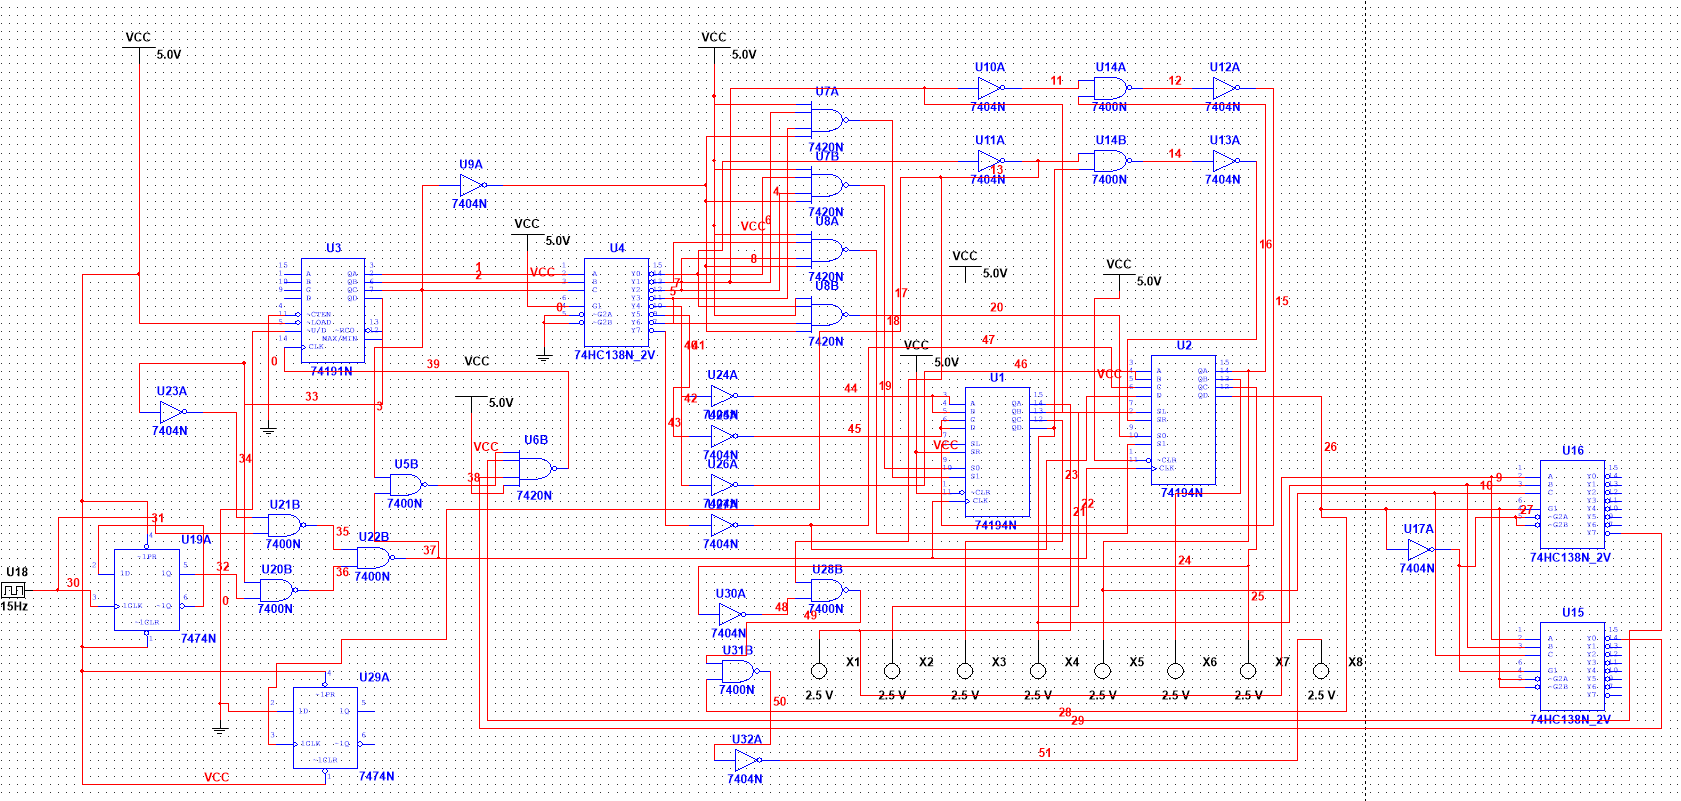
\includegraphics[width=0.99\textwidth]{multisim.png}
    \caption{仿真电路图}
\end{figure}
搭建实物电路。如图是一些状态下的电路截图
\begin{figure}[H]
    \centering
    \begin{minipage}{0.45\textwidth}
    \centering
    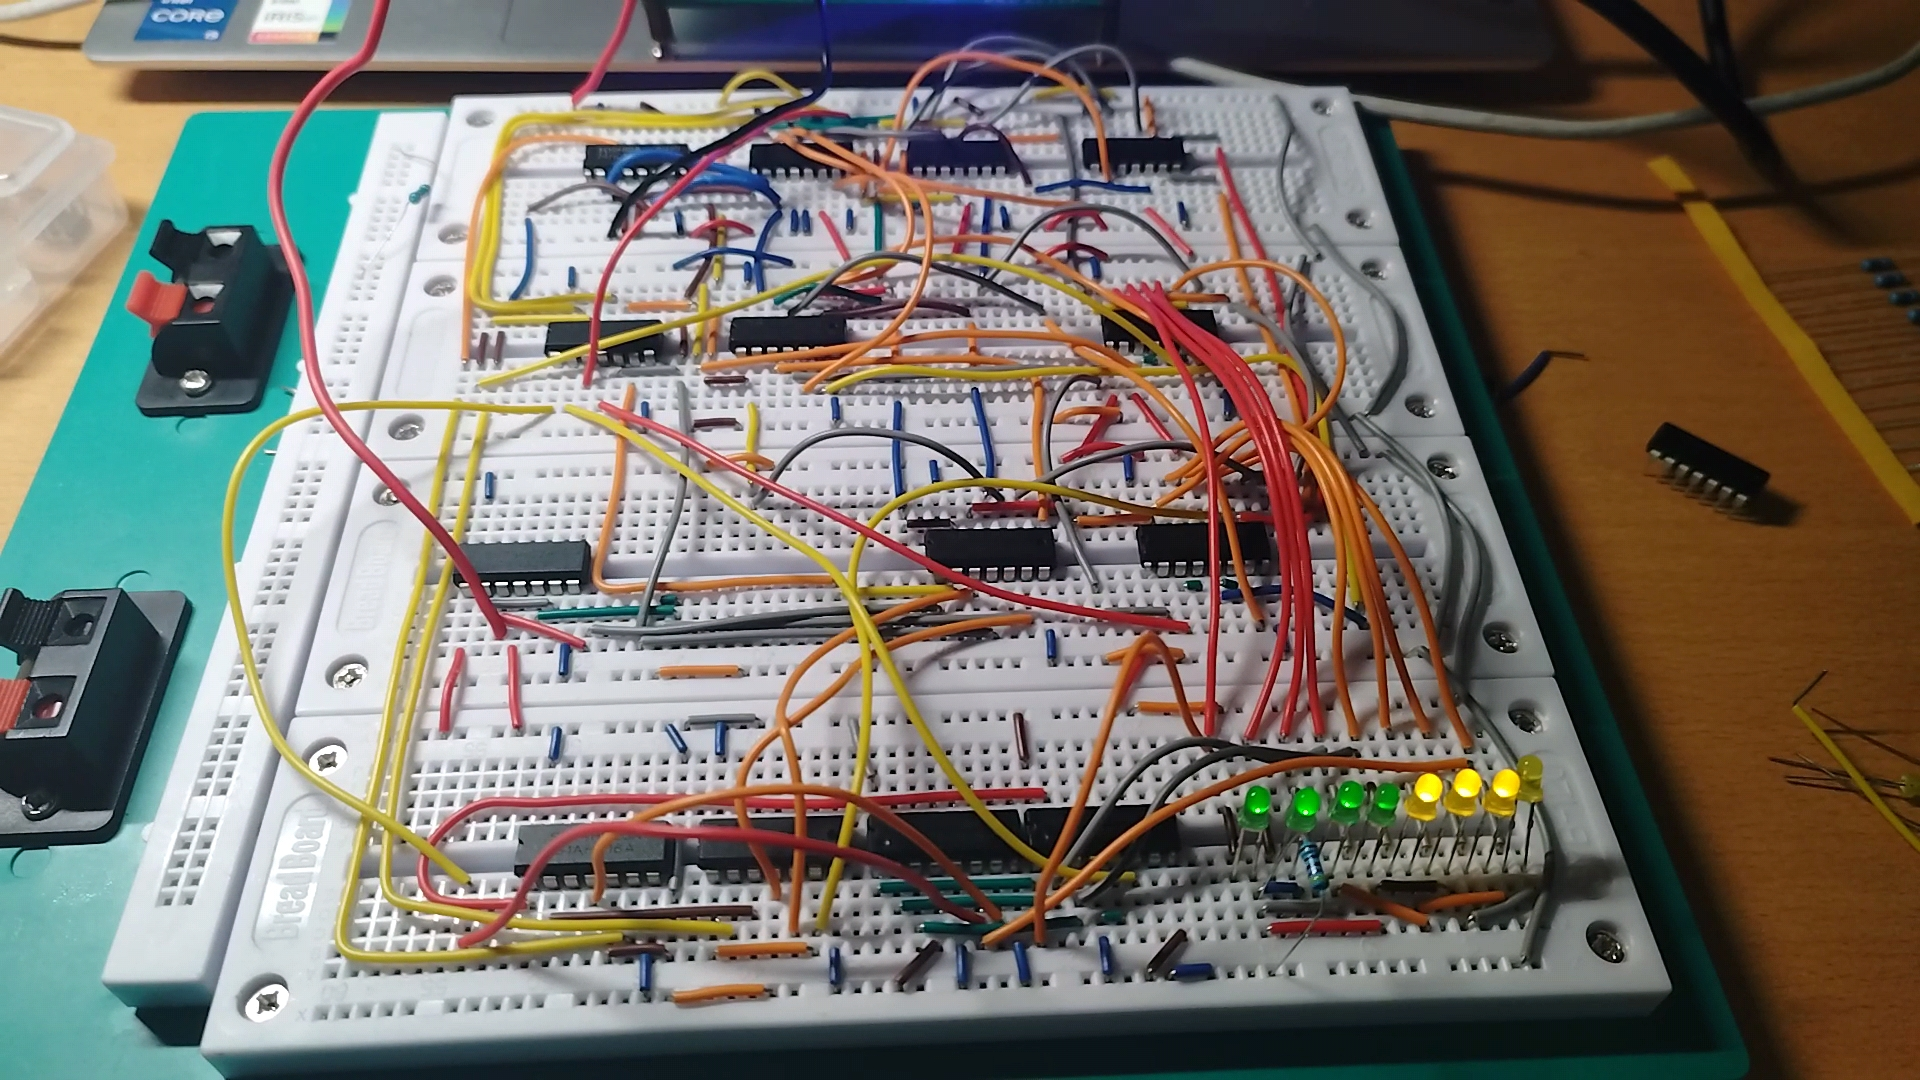
\includegraphics[width=0.9\textwidth]{实物电路图 (1).jpg}
    \caption{实物电路图 (1)}
    \label{}
    \end{minipage}
    \hspace{0.05\textwidth}
    \begin{minipage}{0.45\textwidth}
    \centering
    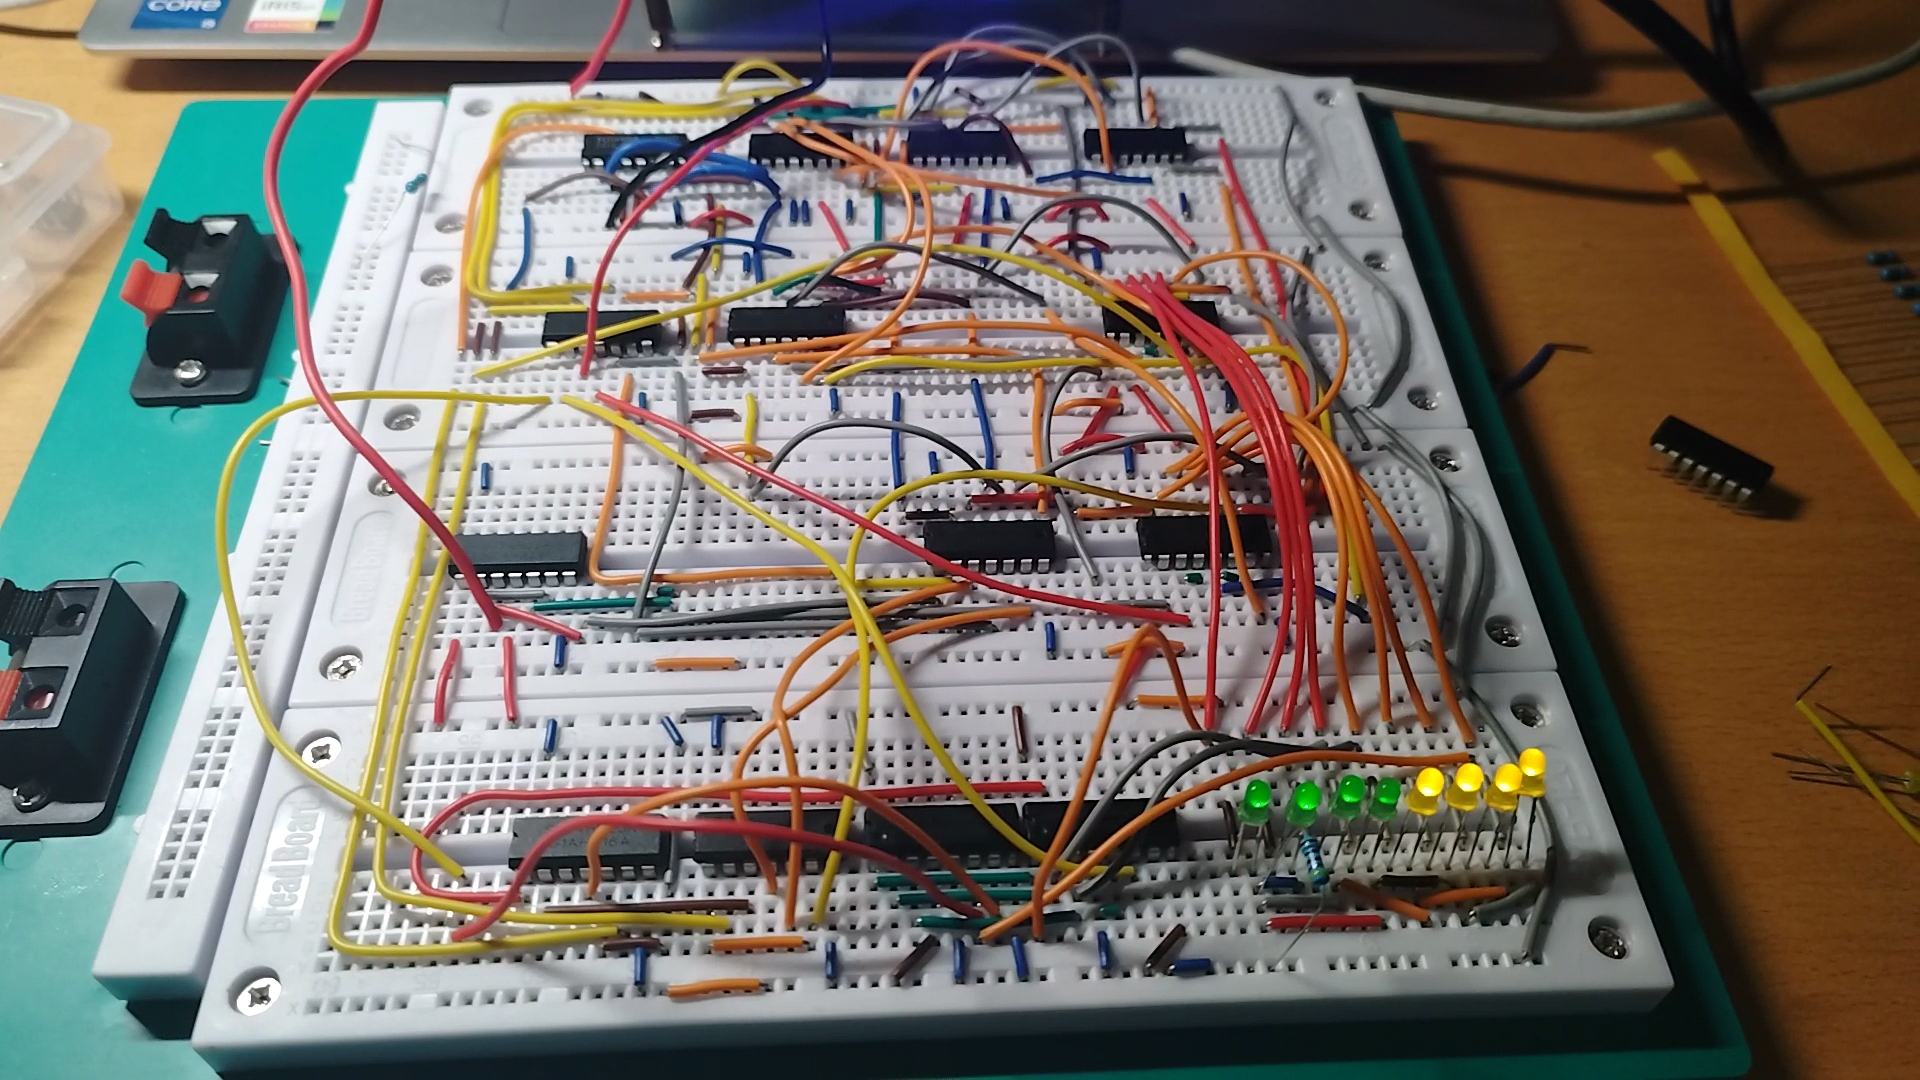
\includegraphics[width=0.9\textwidth]{实物电路图 (2).jpg}
    \caption{实物电路图 (2)}
    \label{7474}
    \end{minipage}
\end{figure}
\begin{figure}[H]
    \centering
    \begin{minipage}{0.45\textwidth}
    \centering
    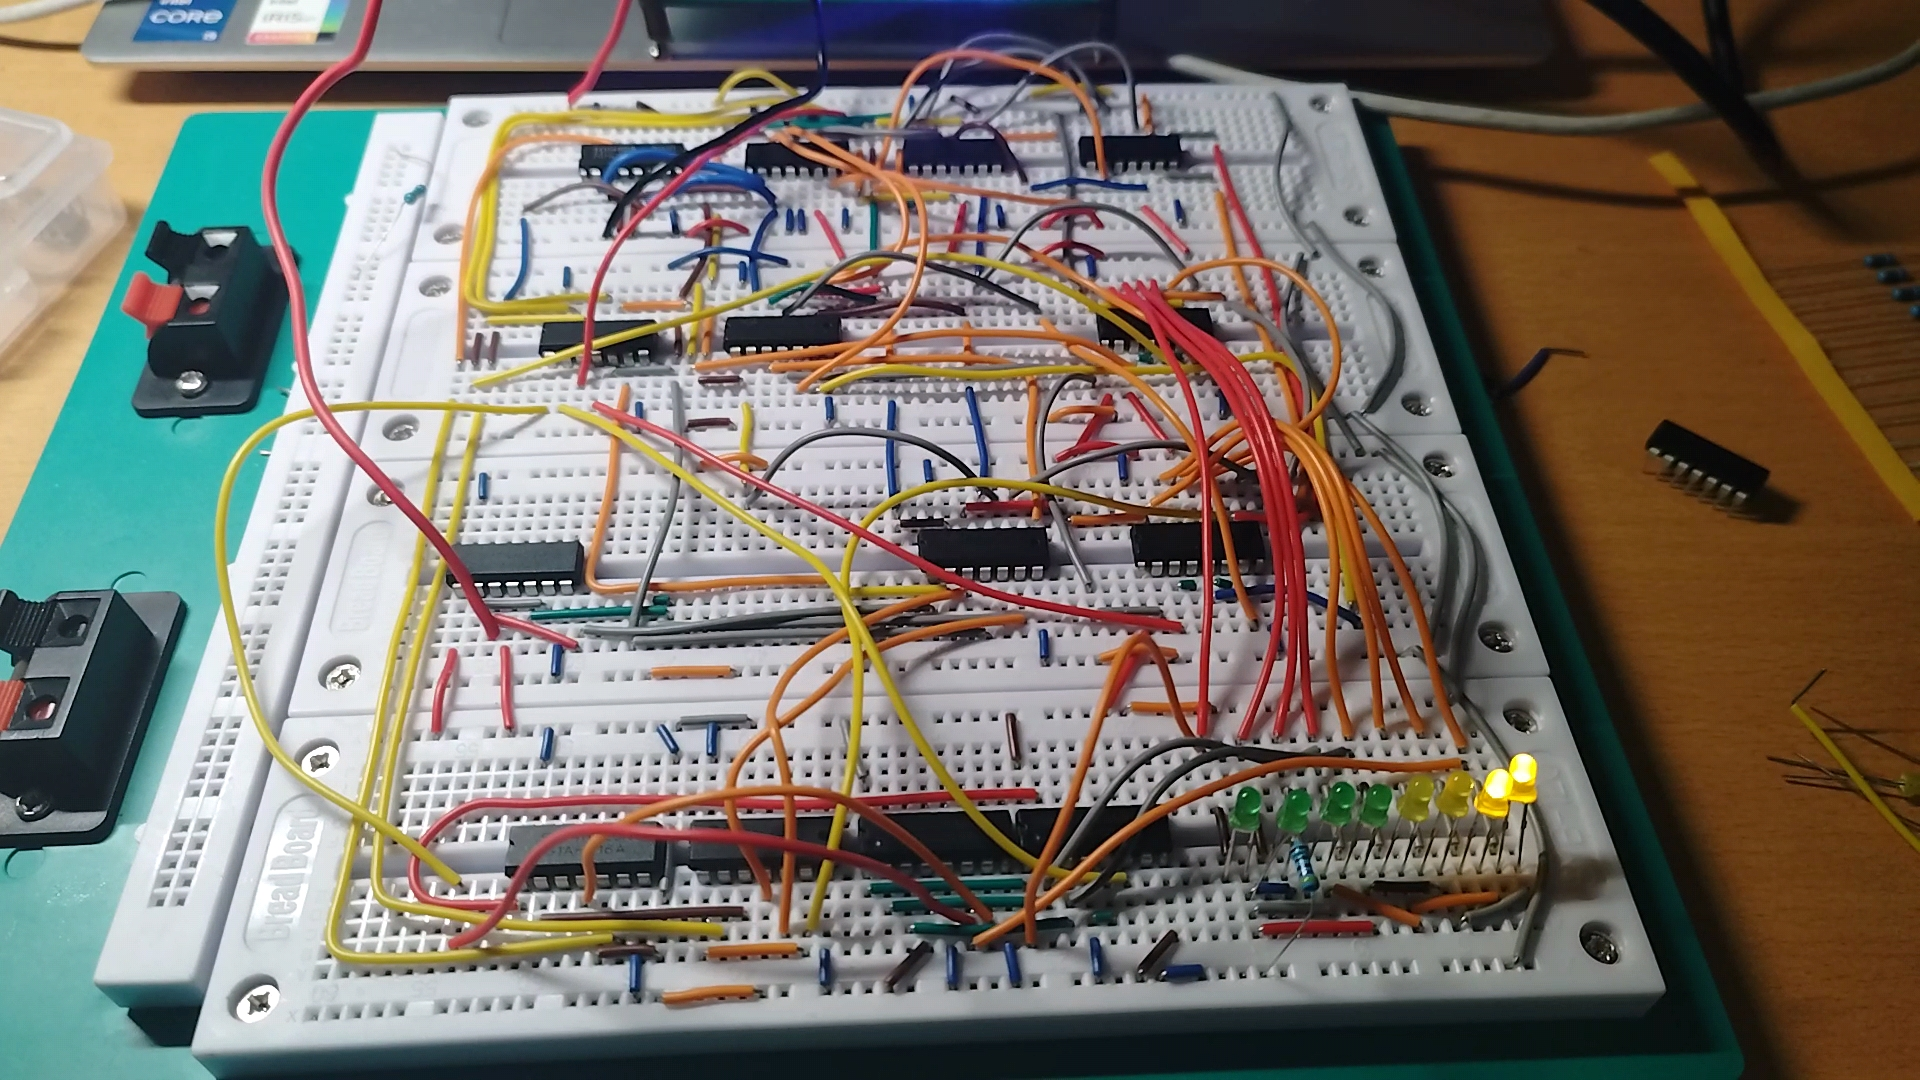
\includegraphics[width=0.9\textwidth]{实物电路图 (3).jpg}
    \caption{实物电路图 (3)}
    \label{}
    \end{minipage}
    \hspace{0.05\textwidth}
    \begin{minipage}{0.45\textwidth}
    \centering
    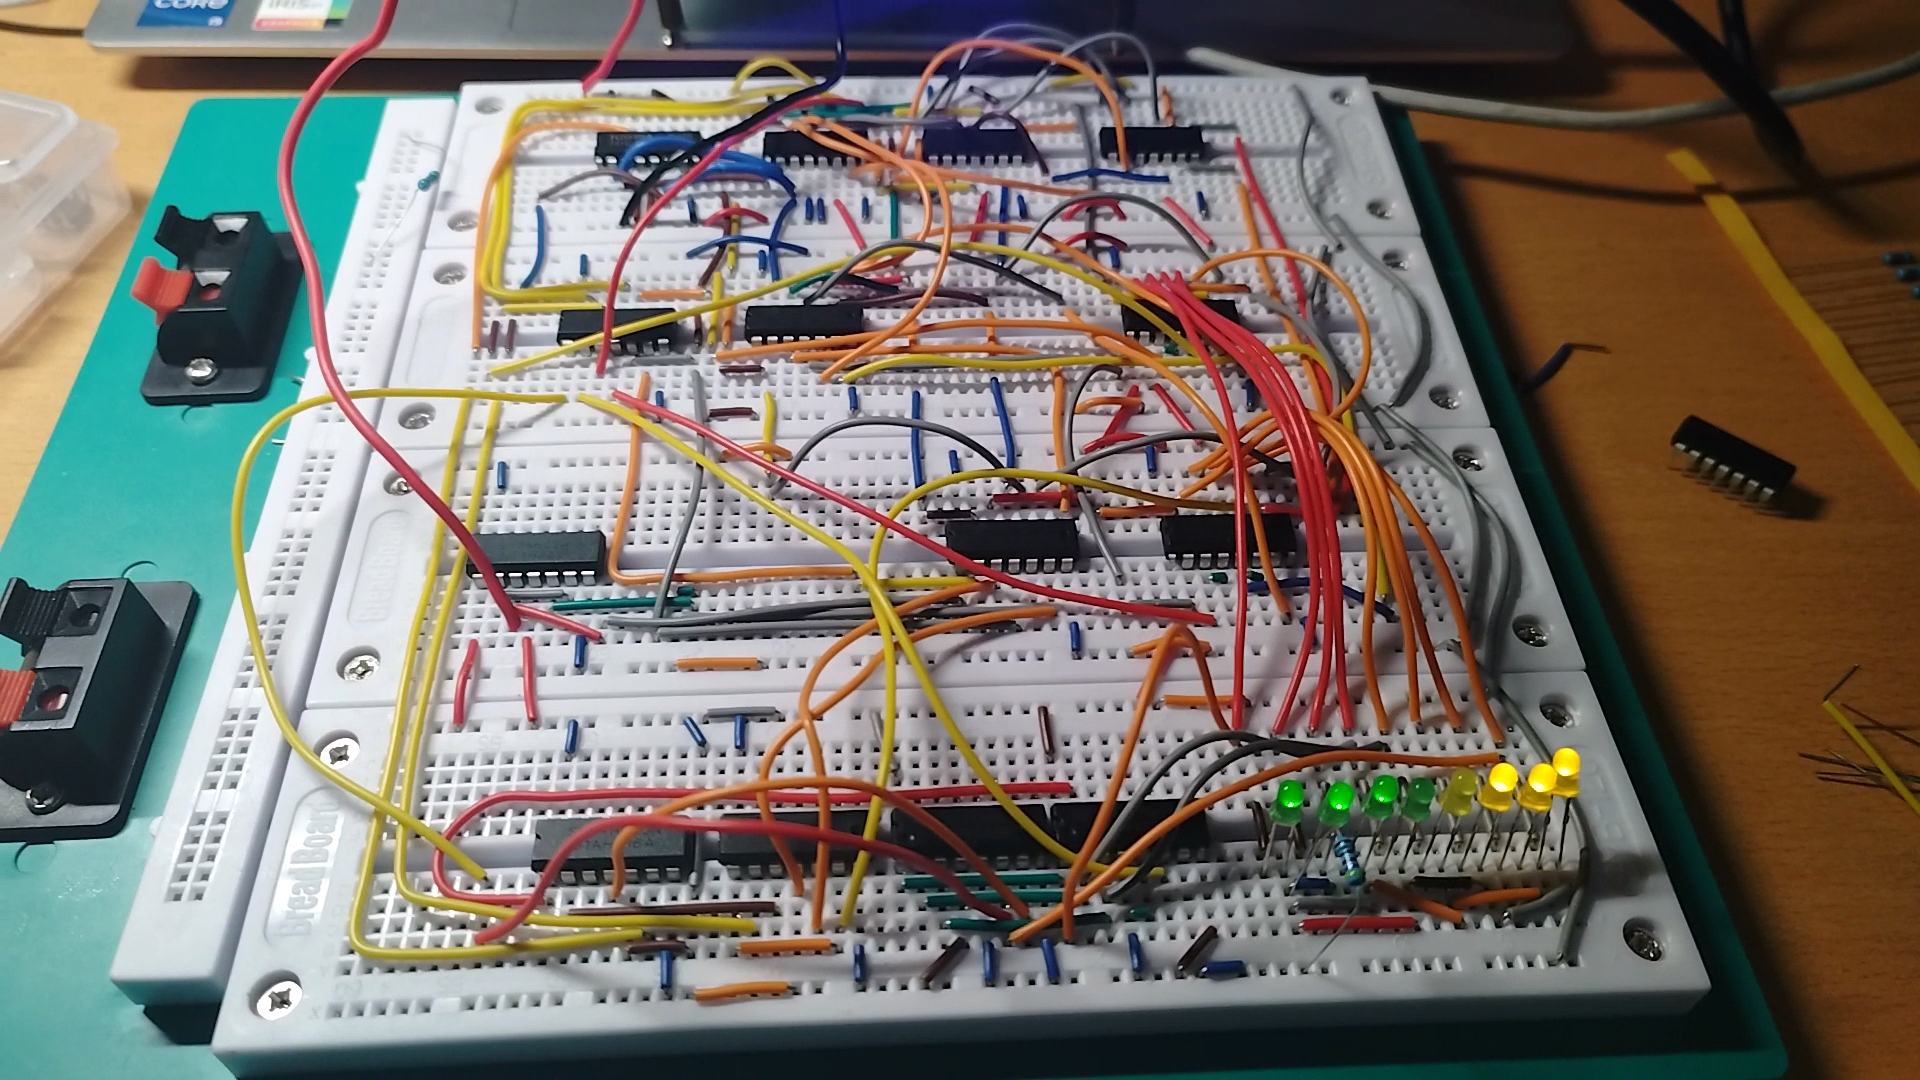
\includegraphics[width=0.9\textwidth]{实物电路图 (4).jpg}
    \caption{实物电路图 (4)}
    \label{7474}
    \end{minipage}
\end{figure}
\section{反思与总结}
本次实物电路的搭建用到很多飞线,这其实对电路的稳定性有影响,也不便于检查错误。但是本实验涉及的芯片数和线路数都很多,如果不飞线会极大地拖慢实验进度,甚至出现线不够用的情况。要想避免飞线,只能从设计开始时重新简化逻辑,减少用线。

在搭建实物电路中遇到一个问题:在以1s/CLK速度运行到花型c的末态时,$L_7$总是不亮,其他状态都正常。首先容易排除的是导线和灯的问题,因为在其他状态下都能正常点亮;其次排除置数端的错误和直接置数功能的缺陷,因为在以0.5s/CLK速度运行到花型c的末态时,$L_7L_8$正常亮;基本上还能排除竞争与冒险的问题,因为接线时$Q_{2C}Q_{2D}$的置数端$C_2 D_2$接在一起且距离很近,并且在以1s/CLK速度运行到花型c的末态时,$L_8$能正常亮。通过检查发现中间有一个与非门的功能异常,换用新的芯片后,所有状态都运行正常。

本次实验还犯了一个错误,即将灯的阴极直接接地。由于LED灯点亮后相当于直接导通,所以输出给灯的信号直接流入地,不能返回前级电路提供反馈导致错误。这一问题通过在灯的阴极接电阻后再接地可以解决。
\end{document}